Um último tipo de detecção de borda apresentado neste trabalho são os detectores de linha \autocite{ref:linedet}. Assim como os operadores baseado em gradiente (seções \ref{sec:sobel} e \ref{sec:grad}), esses filtros dependem de uma certa angulação. No entanto, o direcionamento dentro daquela angulação não é importante. Em especial, o filtro $h_7$ (\ref{fig:h7}) detecta diagonais na linha $y = -x$ e o $h_8$ (\ref{fig:h8}), na linha $y = x$.

\begin{figure}[H]
    \centering
    \begin{subfigure}{0.4\textwidth}
        \centering
        \begin{kmatrix}
    \matrix[square matrix]{
        -1 & -1 & 2 \\
        -1 & 2 & -1 \\
        2 & -1 & -1 \\
    };
\end{kmatrix}
        \caption{~$h_7$}
        \label{fig:h7}
    \end{subfigure}%
    \begin{subfigure}{0.4\textwidth}
        \centering
        \begin{kmatrix}
    \matrix[square matrix]{
        2 & -1 & -1 \\
        -1 & 2 & -1 \\
        -1 & -1 & 2 \\
    };
\end{kmatrix}
        \caption{~$h_8$}
        \label{fig:h8}
    \end{subfigure}

    \caption{Máscaras de detecção de linhas.}
\end{figure}

Podemos ver a diferença com os dois tipos de detectores direcionais comparando com operador Prewitt (\cref{sec:grad}). No caso, as listras das asas da borboleta (veja a original, \cref{fig:sobel:orig}), ficam com a duas bordas bem aparentes. Na \cref{fig:linha:h7}, isso acontece na asa esquerda, enquanto na \cref{fig:linha:h8}, é na asa direita. Agora no operador Prewitt (\cref{fig:grad}), isso não fica aparente em nenhuma das asa, mostrando muitas vezes apenas umas das bordas de cada componente.

\begin{figure}[H]
    \centering
    \begin{subfigure}{0.48\textwidth}
        \centering
        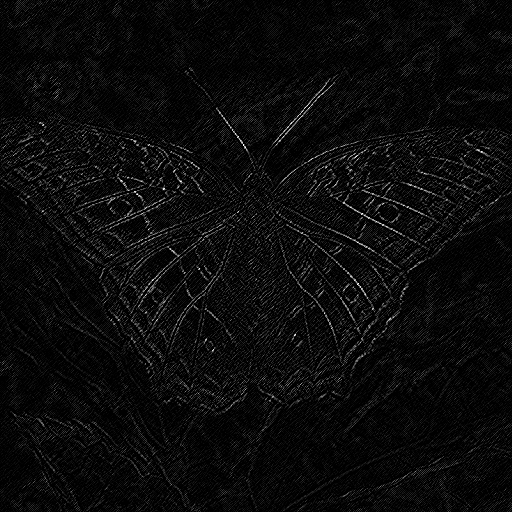
\includegraphics[width=0.9\textwidth]{resultados/butterfly_h7.png}
        \caption{Convolução com $h_7$ (\ref{fig:h7}).}
        \label{fig:linha:h7}
    \end{subfigure}%
    \begin{subfigure}{0.48\textwidth}
        \centering
        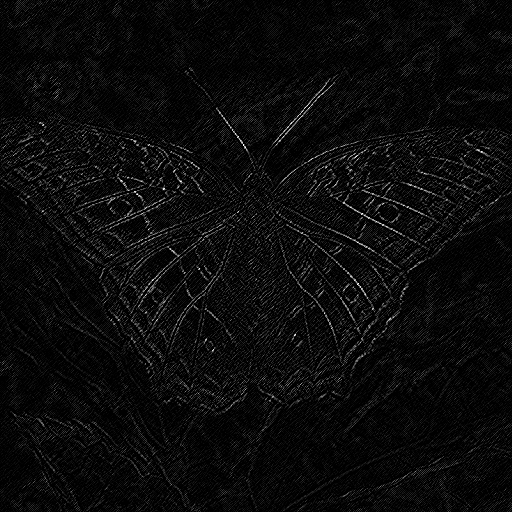
\includegraphics[width=0.9\textwidth]{resultados/butterfly_h8.png}
        \caption{Convolução com $h_8$ (\ref{fig:h8}).}
        \label{fig:linha:h8}
    \end{subfigure}

    \caption{Aplicação dos filtros de detecção de linhas.}
\end{figure}

A aplicação desse filtro pode ser feita com:

\begin{minted}{bash}
    $ python3 main.py imagens/butterfly h7
    # ou
    $ python3 main.py imagens/butterfly h8
\end{minted}
